\subsection{Throw Detection Mechanism}
\label{subsec:throw_detection_mechanism}

To reliably detect a throw, a simple image change detection algorithm is implemented.
It requires a repeated difference computation and therefore a circular buffer is used.

% This section explains the algorithm with its required components and the saving of the images.
This section explains the employed algorithm, its implementation and the saving of the images.

% \subsubsection{Image Change Detection Algorithm}
% \subsubsection{Throw Detection Algorithm}
\subsubsection{Employed Algorithm}
\label{subsubsec:algorithm}
% \todo[inline]{No citations?! Or OpenCV?! Or Baumer?!}

% image change detection algorithm vs throw detection / throw detection mechanism / throw detection algorithm => throw detection employs icda

% Goal of the throw detection is to extract the valid frames of a throw from the continous data stream
  % valid frames have object on them, invalid frames are empty (background)
% real-time
% serial process, 200 fps => >5 ms to process each frame
% not a lot of time for a complex (fancy) algorithm => simplest one possible is used
  % for the throw detection algorithm a simple image change detection algorithm is used

% Algo: computation of the difference and comparison to a threshold to detect changes in the picture

% what this sections describes

% Due to the in section {} mentioned bandwidth limitations of the U3V interface the raw bayer is processed
  % conversion to BGR8 takes too long! => use raw bayer for the detection
% Saving images takes time + unnecessary => saving at the end!
  % see section \ref

% buffers

% frame_id (FID) to keep track of ...
% uses 2 flags and 2 "pointers" to the buffer

% compared against threshold (if mean_diff < threshold, considered to be no change [equal sign])

% throw begin and throw end, what happens

% Why are the last two frames are not valid?
  % only possible to detect the end when there is no change any longer

The goal of the throw detection is to extract valid frames of a throw --- with objects on them --- from the continous data stream of the camera.
Therefore, the throw detection needs to work in real time.
At a frame rate of \SI{200}{fps}, there is $<\SI{5}{ms}$ to process a single frame (without the use of parallel computing).
Due to this time constraint, a simple image change detection algorithm is employed.

\paragraph{Image Change Detection Algorithm}
\vspace{-20pt}
\begin{enumerate}
  \item Compute the absolute difference between the current and the last frame
  \item Compute the average among all the pixels of the difference
  \item Compare the mean difference against a threshold value
\end{enumerate}

This section describes how the throw detection works.
The complete listing of the throw detection can be found in appendix \ref{app:throw_detection}.
The implementation of the image change detection is described in section \ref{subsubsec:image_change_detection}.
Furthermore, the way the threshold value is obtained is documented in section \ref{subsubsec:threshold}.

Due to the bandwidth limitations of the U3V interface mentioned in section \ref{subsubsec:usb3_vision_interface}, the received images are in the raw Bayer pixel format.
A conversion from the Baumer \texttt{BayerRG8} to \texttt{BGR8} takes too long an therefore the raw frames are processed.
Moreover, the valid images are only saved on the hard disk at the end of a throw, as this also takes a lot of time (see section \ref{subsubsec:saving_images}).

For the above reasons, two image buffers are used.
The received images are stored in Baumer \texttt{BGAPI2::Buffer} objects.
To save the images later on, a circular buffer for OpenCV matrices (\texttt{cv::Mat}) is used.
This is documented in section \ref{subsubsec:buffers}.
The size of those image buffers (\texttt{BS}) determines the max. amount of valid frames $N_\text{max}$ that can be captured.

To keep track of the present and past frames, a frame id (\texttt{FID}) is utilized.
Furthermore, two flags are used to mark the beginning and the end of a throw.

Whenever the mean difference between two consecutive frames is greater than or equal to the threshold, they are considered to be different ($\ne$).
Otherwise, the two frames are considered to be equal ($=$).

Once two consecutive frames are different, the flag \texttt{throw\_bgn} is set to \texttt{true} and the current \texttt{FID} is saved in \texttt{throw\_bgn\_idx}.
The current and all subsequent frames --- except for the last two --- belong to the detected throw until two consecutive frames are no longer different.
In this case, the flag \texttt{throw\_end} is set to \texttt{true} and the current \texttt{FID} is saved in \texttt{throw\_end\_idx}.

The last two frames are not valid due to the way the throw detection works.
The first invalid frame occurs when the object leaves the image, as this is still a change in the image and thus not detected.
The second invalid frame results from the fact that the following images are only now the same and therefore the current \texttt{FID} is saved.

Figure \ref{subfig:algorithm_general_case} shows the general case of the just described throw detection.
As already mentioned, the max. amount of valid frames $N_\text{max}$ depends on the image buffer size (\texttt{BS}).
To properly detected a throw, the amount of valid frames $N$ must meet the condition
\[
  N \in \{1..(\text{BS}-2)\}.
\]
In the current implementation, an image buffer size of \SI{1000}{} is used and therefore $N_\text{max} = \SI{998}{frames}$.
An example of three valid frames ($N = 3$) is shown in figure \ref{subfig:algorithm_example_3}.

\begin{figure}[h]
  \centering
  \begin{subfigure}[b]{\textwidth}
    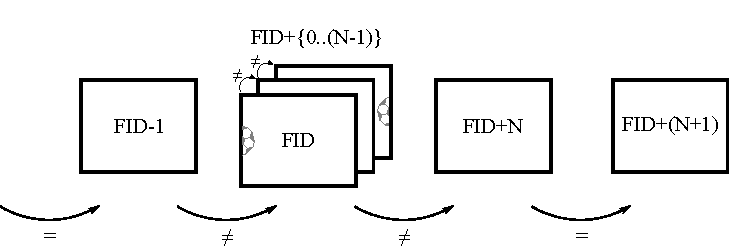
\includegraphics[scale=0.85]{algorithm}
    \caption{General case with $N \in \{1..(\text{BS}-2)\}$}
    \label{subfig:algorithm_general_case}
  \end{subfigure}
  \begin{subfigure}[b]{\textwidth}
    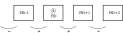
\includegraphics[scale=0.85]{algorithm_ex_1}
    \caption{Example of $N_\text{min} = 1$}
    \label{subfig:algorithm_example_1}
  \end{subfigure}
  \begin{subfigure}[b]{\textwidth}
    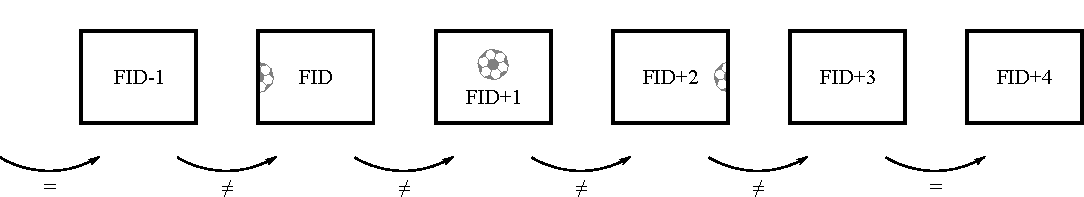
\includegraphics[scale=0.85]{algorithm_ex_3}
    \caption{Example of three valid frames ($N = 3$)}
    \label{subfig:algorithm_example_3}
  \end{subfigure}
  \caption{Illustration of the throw detection}
  \label{fig:throw_detection}
\end{figure}

\subsubsection{Baumer Image Buffer}
\label{subsubsec:baumer_buffer}
% \todo[inline]{Citations}

% Buffer handling by Baumer => large buffer sizes (here not a problem), could be handled by ourselves!
  % handle this by ourselves on the Ultra96 board, due to memory size constrains

\subsubsection{OpenCV Circular Buffer}
\label{subsubsec:opencv_buffer}
% \todo[inline]{Citations}

% OpenCV \texttt{Mat}

% opencv matrix circular buffer (same size as Baumer buffer but shallow [shallow-copy])
  % only pointer to the baumer pixel data
  % copying would require a lot of space and time (which is not much to play with), thus main reason time
% circular buffer graphic

\begin{lstlisting}[style=C++]
  cv_buffer[frame_id % buff_size] = cv::Mat(height, width, CV_8UC1, (void *) pBufferFilled->GetMemPtr());
\end{lstlisting}

\subsubsection{Difference Computation}
\label{subsubsec:difference_computation}
% \todo[inline]{Citations, Picture of how the diff. is calculated or matrices?}

% computation of the difference how it is done with opencv

% done for every frame except the first one (FID = 0)

% after the threshold averaging (see chapter threshold) ?!

\begin{lstlisting}[style=C++]
  cv::absdiff(cv_buffer[frame_id % buff_size], cv_buffer[(frame_id - 1) % buff_size], cv_abs);
  mean_diff = cv::sum(cv_abs)[0] / (width * height);
\end{lstlisting}

\subsubsection{Threshold Value Determination}
\label{subsubsec:threshold}
% \todo[inline]{Citations, Nico is this correct (regarding the 50 Hz flicker)?}

% how is the Threshold Value Determination done:
% average difference to obtain threshold (with pictures)
    % => 50 Hz flicker reduction

\begin{figure}[H]
  \centering
  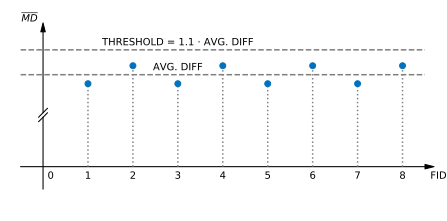
\includegraphics[width=0.75\textwidth]{threshold}
  \caption{Derivation of the threshold value from eigth averaged differences} % 
  \label{fig:threshold}
\end{figure}

\subsubsection{Saving Images}
\label{subsubsec:saving_images}
% \todo[inline]{Citations, Why PNG and not BMP or JPG?}

Resulting in the file names `\texttt{$\{0..(N-1)\}$.png}' (with $N$ beeing the amount of valid frames).

\begin{lstlisting}[style=C++]
  for (int i = throw_bgn_idx; i < (throw_end_idx - 1); ++i) {
    cv::cvtColor(cv_buffer[i % buff_size], cv_transformed, cv::COLOR_BayerBG2BGR);
    cv::imwrite(output_path + std::to_string(i - throw_bgn_idx) + ".png", cv_transformed);
  }
\end{lstlisting}

% https://www.baumer.com/ch/en/service-support/know-how/technical-information-industrial-cameras/baumer-gapi-and-opencv/a/baumer-gapi-and-opencv

